%!TEX root = paper.tex
%related.tex

\section{Related work}
\label{sec:related}

\subsection{Privacy and Government}
This work falls within a line of research that investigates the balance of power between citizens and the state. In~\cite{laskowskigovernment}, we investigated the application of surveillance technology by a government that wishes to remain in power.  Our main takeaway was that enhanced surveillance technology increases incentives for abuse. 

In a similar vein, Goh provides a model of a government that may employ surveillance to lower the risk of a terrorist attack \cite{goh2015prosperity}.  Greater surveillance carries an increased risk that citizens will learn of its existence, which increases the risk that the government loses power.  Goh finds that a rational government will employ less surveillance when citizens value their privacy more, but autocratic governments will employ more surveillance than democratic ones.


\subsection{Privacy and Firms}

Privacy also affects the relationship between citizens and firms, and several strands of research provide insight to this topic.  Privacy can be seen in the classic literature on information economics as an information imbalance between a principal and an agent.  Moral hazard models assume that an agent's actions are not directly observable and the focus is on aligning incentives through contracting \cite{holmstrom1979moral}\cite{stiglitz1981credit}.  In models of adverse selection, agent types are private and certain types are driven out of a market because the principal cannot distinguish between them \cite{akerlof1995market}.  In signaling games, agents may engage in costly actions to signal their private type for economic gain \cite{spence1973job}.  None of these settings correspond to our focus on privacy as protecting a marginalized group.  Furthermore, models in this literature are usually neoclassical in the sense that privacy is an obstacle to maximizing welfare. 

An emerging body of privacy research models the behavior of consumers that participate in two different markets in sequence.  Firms in one market learn about consumers based on their purchase decisions and may be allowed to sell this information to firms in the second market.

In  \cite{johnsoncaviar}, we considered the welfare of consumers as a result of corporate exchanges of personal data.  We found that when consumers are myopic, firms benefit greatly, but consumer surplus is also reduced. When we assume that consumers are strategic, a more complex picture emerges. Consumers are better off in this case, but firms fare worse.  Given that firms actually do in fact share consumer data in ways quite similar to our model, consumers cannot be acting strategically.  One might wonder, if a market for consumer data only exists when consumers are non-strategic, is the market exploiting consumers?  Our current work follows this line of investigation on power imbalances by considering the plight of minority groups targeted by unjust laws.

A final economic literature studies privacy through the lens of mechanism design.  Agents have hidden types and the revelation theorem motivates a focus on mechanisms in which agents report their type directly to the mechanism.  Recently, a set of papers have pioneered the use of differential privacy as a solution concept.  In these models, agents must be approximately truthful to the mechanism and cannot change the outcome by very much if they lie or refuse to participate.  Protecting privacy is not the focus of these models, since the solution concept begins with an assumption that agents don't hide information.

In contrast to the studies we mention, our work distinguishes four distinct types of privacy, which are inspired by technologies and legal debate.  We further apply our model to explore the effects of privacy on divisive laws.

\subsection{Polarization}
Most voters in the United States have been and remain overwhelmingly moderate in their policy positions\cite{layman2006party}. Nevertheless, the United States Congress has passed a number of divisive laws, many of which have been challenged and overturned by the US Supreme Court.  Even in European countries, laws have been passed %xamples in European countries such as France, Belgium, and the Netherlands include laws passed 
against face covering, pejoratively dubbed ``burka bans.''

\begin{figure}[htbp]
\begin{center}
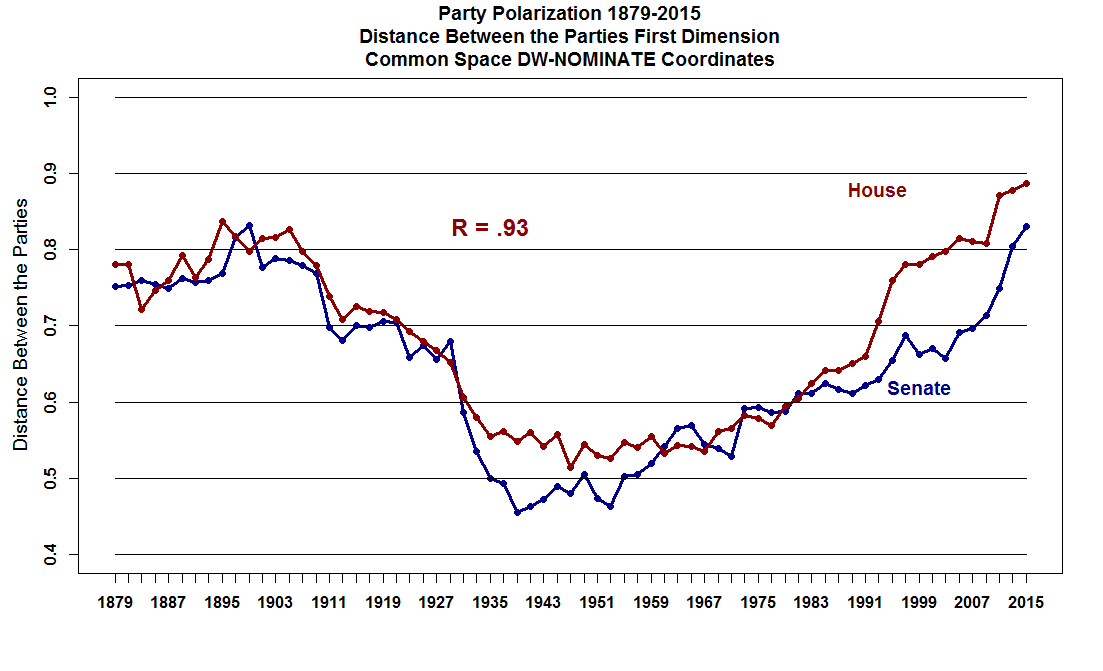
\includegraphics[width=0.4\textwidth]{figs/polar_house_and_senate_46-115_july_11}
\caption{{\bf Polarization Trends in the US Congress}}
\label{fig:uscongress}
\end{center}
\end{figure}

The United States congress in particular has become increasingly polarized over the last 40 years (see Figure \ref{fig:uscongress}); and
researchers have posited a number of reasons for this phenomenon \cite{barber2015causes}\cite{poole1984polarization}, ranging from a polarized electorate, to southern realignment, to gerrymandering, to the evolution of modern primary elections, to economic inequality, to money in politics, to the media environment, or to congress-based factors such as congressional rule changes, majority party agenda control, party pressures, teamsmanship, or the breakdown of bipartisan norms.  All of these issues are discussed in~\cite{poole1984polarization}.
More culturally-specific theories involving authoritarianism are also prevalent \cite{hetherington2009authoritarianism}; and there is a remarkably close correlation between economic
inequality and polarization in the United States~\cite{mccarty2006polarized}.  See Figure \ref{fig:inequality}.

\begin{figure}[htbp]
\begin{center}
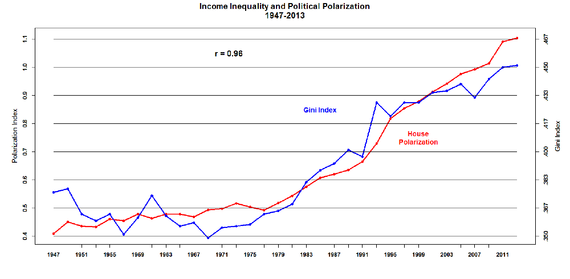
\includegraphics[width=0.4\textwidth]{figs/8141eb7a0}
\caption{{\bf Polarization versus Income Inequality}}
\label{fig:inequality}
\end{center}
\end{figure}


A more economically-driven explanation derives from the notion of information cascades. An information cascade occurs when people receive a noisy signal and rely on friends and colleagues to distill the essential parts.  According to \cite{bikhchandani1992theory},
``An information cascade occurs when it is optimal for an individual, having observed the actions of those ahead of him, to follow the behavior of the preceding individual without regard to his own information." 

The notion that people exhibit herding behavior in predictable circumstances has been around for decades \cite{shiller1995conversation}.  For example, researchers at Iowa State University conducted 259 interviews with farmers who had largely refused offers to adopt drought-resistant seed corn during the Great Depression and Dust Bowl.  They found that the slow rate of adoption was due to ``how farmers valued the opinion of their friends and neighbors instead of the word of a salesman''\cite{beal1957diffusion}.



We include this notion of influenced behavior in our model as a way to explain the source of divisiveness.  Our model does not mandate any herd behavior, but merely allows it.  This allowance appears justified by the observation that the United States has a legislative system that is organized like Figure \ref{fig:partisonship}, while it has an electorate that is more like Figure \ref{fig:voters}.


\begin{figure}[htbp]
\begin{center}
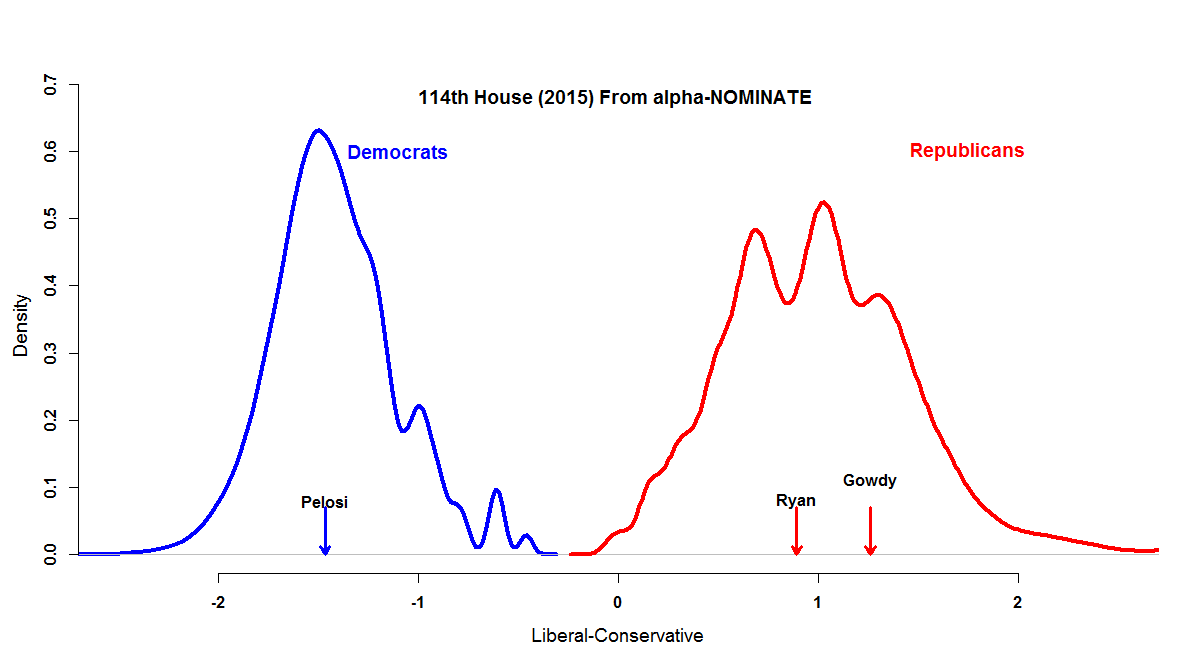
\includegraphics[width=0.4\textwidth]{figs/alpha_House_114_Histogram_8_January_2016}
\caption{{\bf Partisonship in the US House of Representatives}}
\label{fig:partisonship}
\end{center}
\end{figure}




\begin{figure}[htbp]
\begin{center}
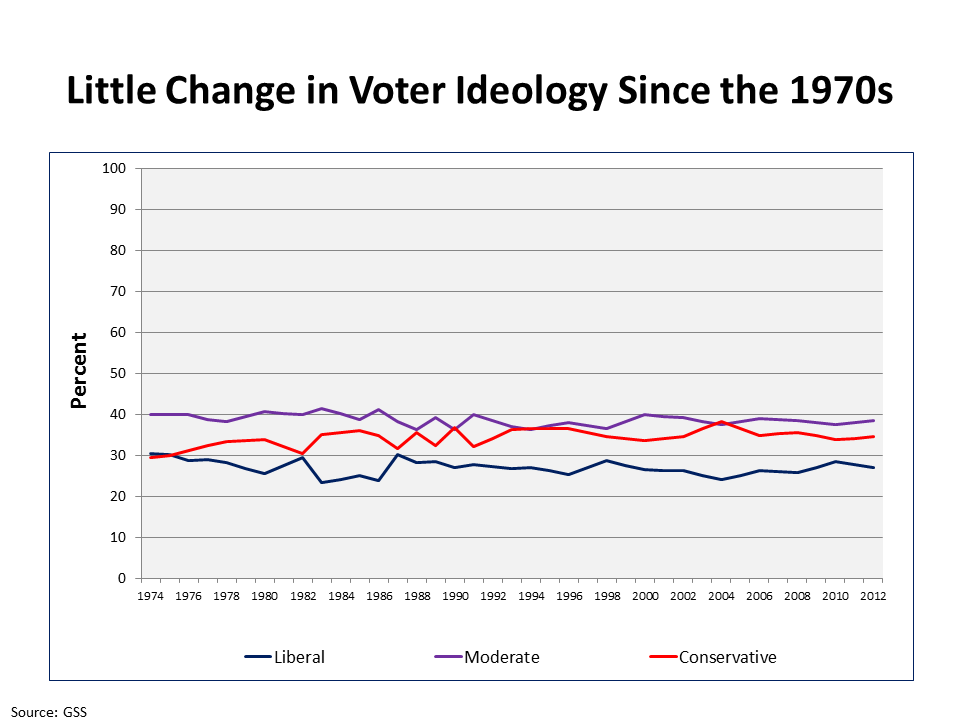
\includegraphics[width=0.4\textwidth]{figs/polarization2}
\caption{{\bf Long Term Trends in US Voter Ideology}}
\label{fig:voters}
\end{center}
\end{figure}



